Certainly! Below is a TikZ LaTeX code that generates a Penrose diagram for both cases you described:

```latex
\documentclass{article}
\usepackage{tikz}

\begin{document}

\section*{Penrose Diagrams}

\subsection*{Case 1: $\pi/2 < \tau_0 < \pi$}

\begin{figure}[h]
    \centering
    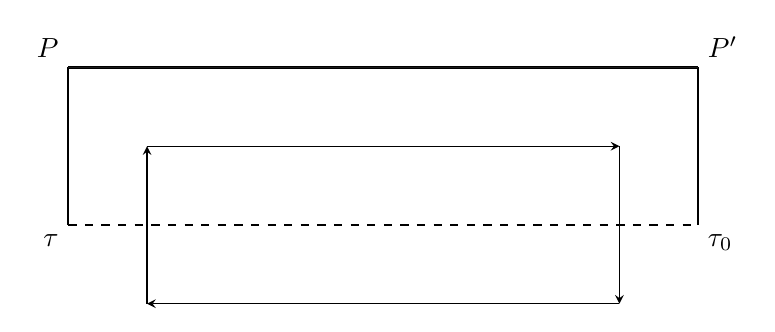
\begin{tikzpicture}[scale=2]
        % Draw the horizontal lines
        \draw[thick] (-2,0) -- (2,0);
        \draw[dashed, thick] (-2,-1) -- (2,-1);
        
        % Draw the vertical lines
        \draw[thick] (-2,0) -- (-2,-1);
        \draw[thick] (2,0) -- (2,-1);
        
        % Label the points
        \node[above left] at (-2,0) {$P$};
        \node[below left] at (-2,-1) {$\tau$};
        \node[above right] at (2,0) {$P'$};
        \node[below right] at (2,-1) {$\tau_0$};
        
        % Shaded region
        \fill[gray!30] (-2,0) rectangle (2,0);
        
        % Draw the null cones
        \draw[-stealth] (-1.5,-0.5) -- (1.5,-0.5);
        \draw[-stealth] (1.5,-0.5) -- (1.5,-1.5);
        \draw[-stealth] (1.5,-1.5) -- (-1.5,-1.5);
        \draw[-stealth] (-1.5,-1.5) -- (-1.5,-0.5);
    \end{tikzpicture}
    \caption{Penrose Diagram for $\pi/2 < \tau_0 < \pi$}
\end{figure}

\subsection*{Case 2: $\tau_0 > \pi$}

\begin{figure}[h]
    \centering
    \begin{tikzpicture}[scale=2]
        % Draw the horizontal lines
        \draw[thick] (-2,0) -- (2,0);
        \draw[d